\documentclass[a4paper,oneside,12pt]{report}
\usepackage{styles/fbe_tez}
\usepackage[utf8x]{inputenc}
\renewcommand{\labelenumi}{(\roman{enumi})}
\usepackage{amsmath, amsthm, amssymb}
\usepackage[bottom]{footmisc}
\usepackage{cite}
\usepackage{url}
\usepackage{graphicx}
\usepackage{longtable}
\graphicspath{{figures/}}
\usepackage{multirow}
\usepackage{subfigure}
\usepackage{comment} % for multiline comment
\usepackage{tabularx} % better table formatting
\usepackage{array} % for column type customization
\usepackage{float} % for [H] placement on figures - not to wrap figures to the next page for the sake of optimized text flow. with this structure we are using in, figures are being replaced on the exact place as they are in the text flow.


\begin{document}

\chapter{Introduction}

When we started this research, we asked ourselves a simple question: why do "smart" cities often feel so disconnected from the people who actually live in them? We see technology everywhere (sensors in our buildings, digital twins of our cities, and massive data centers managing national infrastructure). But despite all this tech, there seems to be a missing link. The person in the wheelchair trying to navigate a steep ramp, or the community trying to report a water leak, often feels like an afterthought in these grand digital systems.

Our goal in this term paper is to explore how we can bridge this gap. We don't want to just build another technical system; we want to find a way to make these environments "inclusive" and "participatory." We believe that a smart environment shouldn't just be about efficiency; it should be about connection (connecting buildings to cities, cities to nations, and most importantly, connecting people to the decisions that shape their world).

In this report, we try to piece together a solution. We looked at a lot of different research (from high-level theories about co-creation to very specific technical papers about coding compliance rules). What we found was that while the pieces of the puzzle exist, they aren't really talking to each other. Our proposed framework is our humble attempt to put those pieces together into something that might actually work.

\chapter{Problem Definition}

As we dug deeper into the literature, a clear problem started to emerge. It wasn't that we lack the technology; it's that the technology and the people are in two different worlds.

On one side, we have the visionaries like Sanders\cite{Sanders2008} and Wilson\cite{Wilson2015}. They tell us that for a design to be successful, users need to be partners. They warn us that if we treat people as passive subjects, we end up with "smart" homes that people actually hate living in. This made a lot of sense to us. But on the other side, we have the technical experts. Researchers like Dave\cite{Dave2018} and Liciotti\cite{Liciotti2020} are doing amazing work connecting BIM models to IoT sensors and using artificial intelligence to understand human activity. But their work is often very focused on the "how" (how to get the data, how to process it) and less on the "who."

We noticed a "silo" (Dave et al.\cite{Dave2018} uses this word) problem. The building experts are solving building problems. The urban planners are solving city problems. And the national infrastructure teams are dealing with their own massive networks. But a water leak doesn't care about these boundaries. It starts in a building, flows into the city network, and affects the national resource. Currently, these systems don't really talk to each other.

Furthermore, even when we have standards like IFC for buildings, they are often used just for geometry, not for the kind of rich, participatory data we care about. We realized that if we want a truly inclusive smart environment, we need to break down these silos. We need a way to connect the "participation" that Sanders talks about with the "technical implementation" that Dave builds, and we need to do it across all scales (from the room you're sitting in to the country you live in).

\chapter{Literature Review}

To understand how to solve this, we looked at nine key papers (actually one of them is a government project (Ofwat's project\cite{ThamesWater2024})). We tried to group them not just by date, but by what they actually taught us.

\section{The "Why": Participation and User Needs}
Everything starts with the user. Sanders' research\cite{Sanders2008} was a real eye-opener for us. They argue that we need to move from "user-centered design" to "co-creation." It's not enough to just watch people; we have to invite them to the design table. This gave us the theoretical backbone for our project: users are experts in their own lives.

Then we read Wilson's research\cite{Wilson2015}, and it was a bit of a reality check. They analyzed smart homes and found that they often fail because they ignore the complex, messy reality of family life. They showed us that "smart" doesn't always mean "helpful." This reinforced our belief that technology needs to be flexible and sensitive to how people actually live.

\section{The "How": Technical Foundations}
Once we understood the human need, we looked for the technical tools. Dave\cite{Dave2018} provided a crucial piece of the puzzle. They showed us how to integrate BIM (Building Information Modeling) with IoT (Internet of Things). This is how we can make a static building model "alive" with real-time data. It's the bridge between the physical walls and the digital signals.

Liciotti\cite{Liciotti2020} took it a step further. They used unsupervised learning to detect activities in a smart home. What struck us here was the potential for the house to "understand" what's happening without needing invasive cameras everywhere. It suggests that we can have smarts without sacrificing privacy, which is a big concern for us.

\section{The "Scale": From Buildings to Nations}
But we can't just stay inside the house. Mendonça\cite{Mendonca2024} showed us a really cool way to automate rule checking using IDS (Information Delivery Specification). They used it to check if a building meets accessibility standards. We thought, "Wow, this is how we translate a human rule (like 'door must be wide') into something a computer can check automatically."

Then Zhou\cite{Zhou2024} zoomed out to the city level. They talked about the "Quadruple Helix" (bringing together government, industry, academia, and citizens). It made us realize that our framework needs to support this kind of broad collaboration.

Finally, we looked at the Ofwat's\cite{ThamesWater2024} project. This was different because it's a real-world, national-scale infrastructure project. They are using open data and graph databases to manage water networks. It showed us that this isn't just academic theory; big organizations are actually trying to solve these data integration problems right now.

\section{The "Gap": Recent Attempts and Challenges}
We also looked at some very recent work to see what's happening right now. Aavild\cite{Aavild2024} tackled the hardware problem. They showed that running everything on a single Raspberry Pi is a bad idea and proposed a distributed system. This is practical advice for us: don't overload the local controller.

Adreani\cite{Adreani2024} built a "Digital Twin" for a smart city. It's an impressive system, but we felt it was still a bit top-down. It gathers data from everywhere, but we wondered: where is the user in that massive dashboard? This confirmed to us that while the "Digital Twin" technology is maturing, the "Participatory" part is still lagging behind.

\chapter{Proposed Conceptual Framework}

Based on all this reading, we tried to come up with a framework that ties it all together. We call it the \textbf{Inclusive Participatory Smart Environments Framework}.

\section{The Three Scales}
We realized that you can't solve this problem at just one level. Our framework is organized into three distinct scales:

\begin{itemize}
    \item \textbf{Building Scale (The Home):} This is where researches of Dave\cite{Dave2018} and Liciotti\cite{Liciotti2020} live. It's about the immediate environment—sensors, BIM models, and local feedback. It's personal and private.
    \item \textbf{Urban Scale (The City):} This is the neighborhood level. It's where Adreani\cite{Adreani2024}'s Snap4City platform comes in. It connects multiple buildings and public spaces.
    \item \textbf{National Scale (The Infrastructure):} This is the big picture. It includes the physical networks like the Ofwat project\cite{ThamesWater2024}, but also the strategic governance (where Zhou\cite{Zhou2024}'s Quadruple Helix model ensures government and citizens are actually talking to each other).
\end{itemize}

\section{The Cross-Cutting Layers}
But these scales shouldn't be silos. So, we propose vertical layers that cut through all of them:

\begin{itemize}
    \item \textbf{Participation Layer:} Inspired by Sanders\cite{Sanders2008}, this layer ensures that at every scale, there is a way for people to give feedback. Whether it's adjusting a thermostat or voting on a new park, the user is involved.
    \item \textbf{Data Layer:} This is the plumbing. It uses the graph technologies and open standards we saw in Ofwat project\cite{ThamesWater2024} to make sure data flows smoothly from the sensor to the national database.
    \item \textbf{Governance Layer:} This defines the rules (like the accessibility checks from Mendonça's research\cite{Mendonca2024}). It ensures that the system is safe, fair, and compliant.
\end{itemize}

\section{The Internal Agent}
One thing we worried about was: what if the internet goes down? Or what if the central server is too slow? That's why we added the concept of an \textbf{Internal Agent}.

This is a local "brain" that lives at the Building Scale. It doesn't need the cloud to make safety-critical decisions. If a fire alarm goes off, or a gas leak is detected, the Internal Agent acts immediately. It listens to the local sensors and follows the local rules. It only talks to the upper layers when it needs to share long-term data or get updates. We think this makes the system much more resilient and responsive.

\begin{figure}[H]
    \centering
    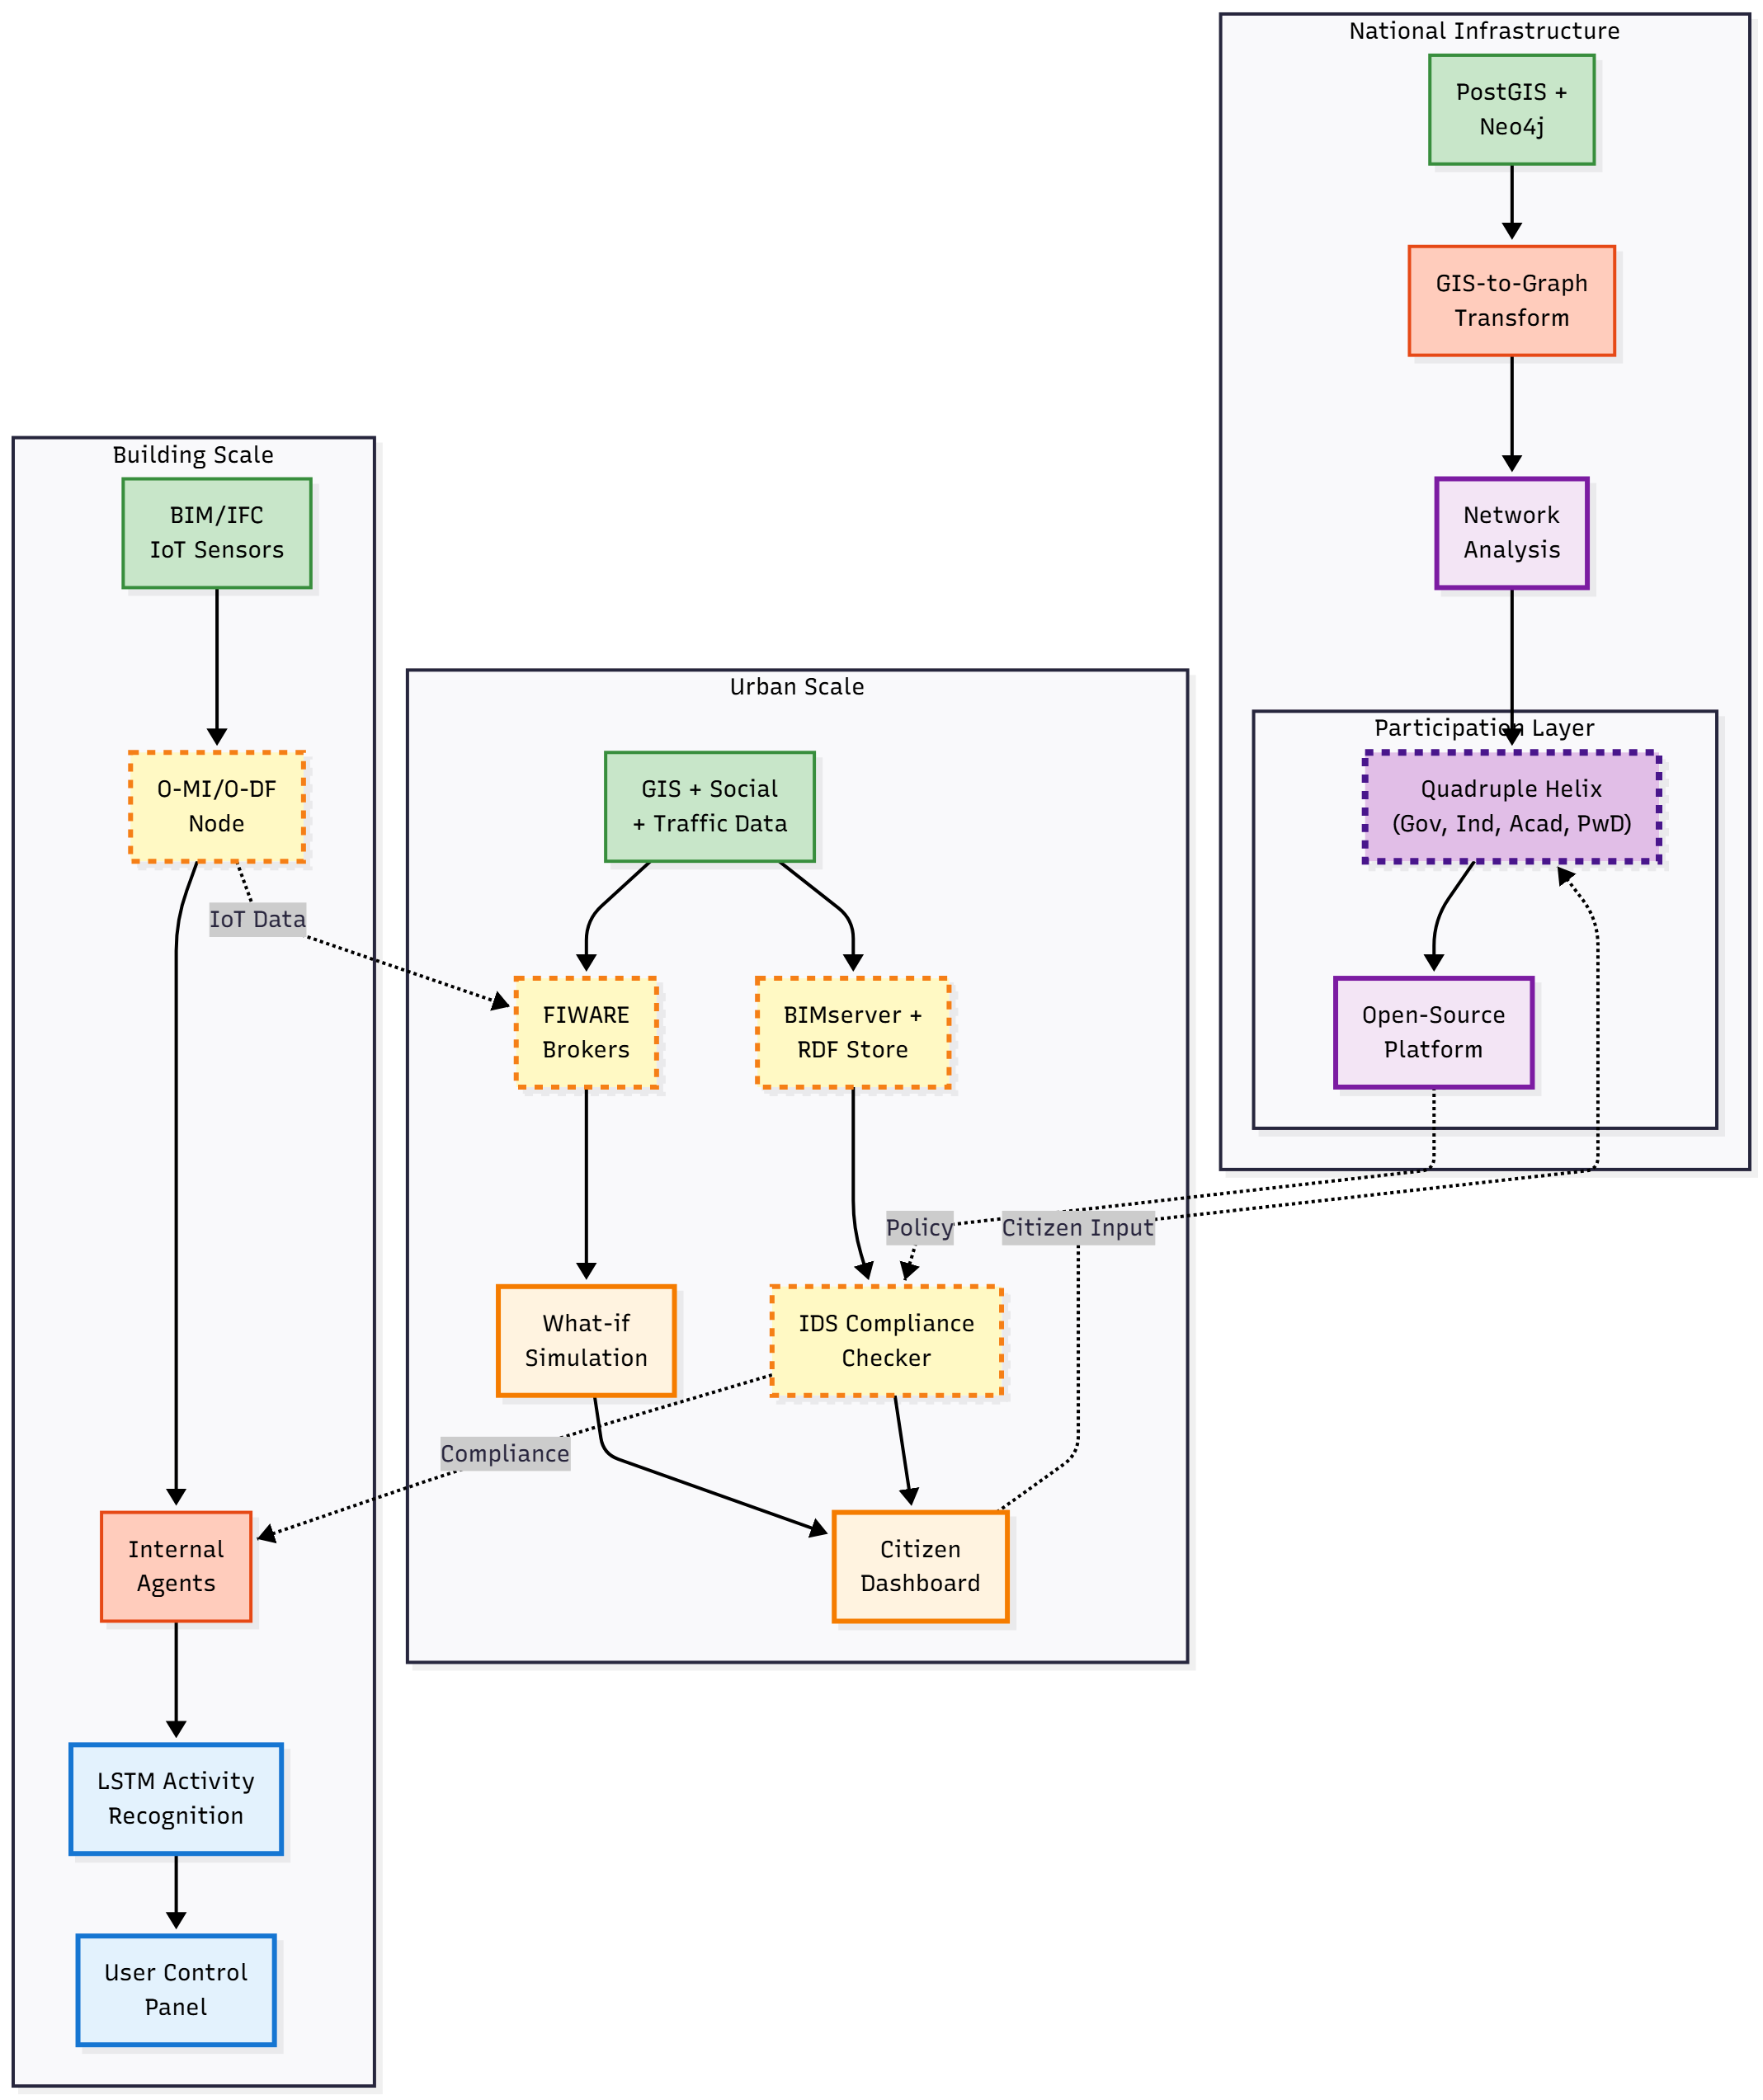
\includegraphics[width=\textwidth]{our-framework-proposal-vertical.png}
    \caption{Our proposed Inclusive Participatory Smart Environments Framework, showing the interaction between the three scales and the cross-cutting layers.}
    \label{fig:framework}
\end{figure}

We believe this structure gives us the best of both worlds: the efficiency of a connected smart city and the resilience and human-centric focus of a participatory home.


% ===============================
% REFERENCES
% ===============================
\bibliographystyle{styles/fbe_tez_v11}
\bibliography{references}
\end{document}
